\section{Simulation Analysis}
\label{sec:simulation}
Since the input voltage source in this circuit is sinusoidal, the voltage and current values of the various components vary in time, and we are interested therefore in analysing how they evolve in time and obviously we want to picture the transformation of our AC input voltage source from the input to the output of the circuit. We will run a transient analysis which will help us measuring the input and output impedances. We will also run a frequency response analysis in order to determine the gain and central frequency of our output amplified sinusoidal signal.

\subsection{Frequency response and impedances}
We measured the input impedance of the circuit, seen through the perspective of the source, and the output impedance, seen through the perspective of our output (using a dummy test source). With the frequency response, we measured the voltage gain in our output and the lower and upper cut-off frequencies. Using the same equation from the theoretical analysis we determined the central frequency, then extracting the output gain for such frequency. In table~\ref{tab:main}, we present the results of our calculations. In figures~\ref{fig:gainstage}and~\ref{fig:outputstage} we can see the frequency response for our output's gain and phase, respectively. With this figures we can notice a slightly narrow band-pass filter, as expected and wanted. Regarding the phase plot though, we notice a full circle phase drop until it reaches the 90 degrees back again, whereas in the theoretical analysis the phase drops from 90 degrees to -90 degrees, stabilizing there. This difference is cause of the aproximation used to study the OP-AMP behaviour in the theoretical section. For study purposes, we considered the OP-AMP did not introduce any phase difference in its output compared to its input, which is not true in reality. Due to the two transistors used in the uA741 OP-AMP, the transfer function in this sector actually presents 2 poles, which causes a double phase drop of 90 degrees (45 degrees the decade before and 45 degrees the decade after) each, which then means the phase actually drops 180 degrees due to the OP-AMP, hence stabilizing not in -90 degrees, but in 90 (-270) degrees.

\begin{table}[h]
  \centering
  \begin{tabular}{|l|r|}
    \hline    
    {\bf Name} & {\bf Values} \\ \hline
    @$V_{DC}$ & 12.000000 \\ \hline 
@$V_{ACripple}$ & 0.000015 \\ \hline 
Cost & 1902.400000 \\ \hline 
Merit & 33.573648 \\ \hline 

    \input{outimp_tab}     
  \end{tabular}
  \caption{Output gain, center frequency, and input and output impedances of the OP-AMP band-pass filter.}
  \label{tab:main}
\end{table}

Our input impedance value is reasonably high, so, depending on the input signal's inner resistance, it does allow the great majority of the input voltage to flow through ahead to the OP-AMP. That being said, the output impedance value is also considerably high, which in this case is not desirable. This means that for loads with low resistance values, most of the voltage will be consumed by the circuit's output impedance itself, undoing its very purpose. This band-pass filter is then better suited for loads with greater resistance values. Given the components we had at our disposal, it was very difficult to accomplish a lower value for the output impedance, specially without comprimising the most important goal of this laboratory assignment.
Looking now to the central frequency obtained, and the gain for such frequency, we had very slight deviations from the targeted values - 1 kHz and 40 dB. That being said, we obtained a 1.863\% relative error for the central frequency value, and a 0.264\% error for the output voltage gain, which we consider to be fantastic results, when we take into account the limited components available, which made optimization more difficult than usual.

\begin{figure}[h!] \centering
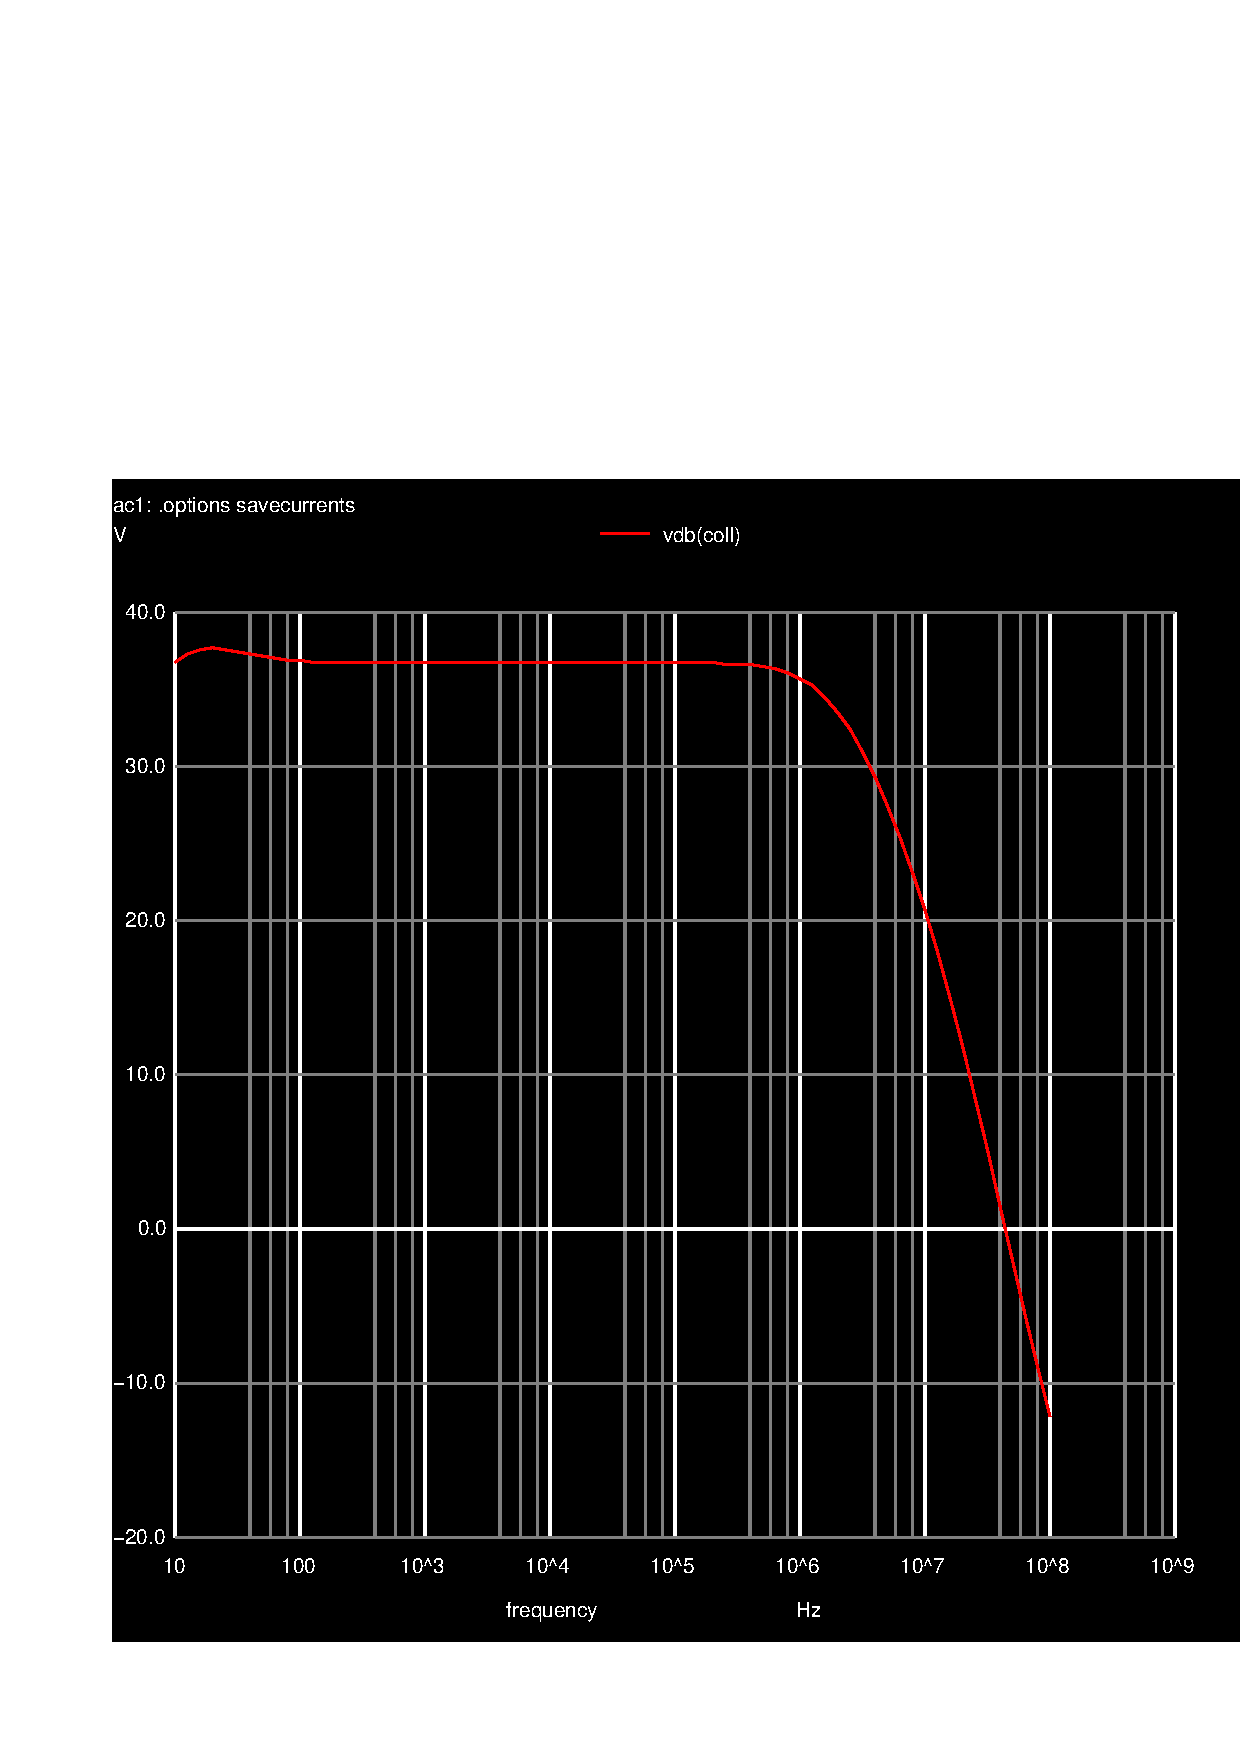
\includegraphics[width=0.6\linewidth]{vo1f.pdf}
\caption{Output voltage gain (frequency response).}
\label{fig:gainstage}
\end{figure}

\begin{figure}[h!] \centering
\includegraphics[width=0.6\linewidth]{vo1p.pdf}
\caption{Output voltage phase difference (frequency response).}
\label{fig:outputstage}
\end{figure}

\subsection{Final product and merit}
In figure~\ref{fig:comp}, we can compare the output signal to the input. As normal, the output voltage does not possess a DC component. Since the wanted gain was 40 dB, which is the same as 100$\times$ the initial amplitude, we can see the clear evolution from the starting 10mV to the final 1V of amplitude (more or less). For the first few milisseconds there is some small variation in the output sinusoidal wave due to a small transient regime.
In table~\ref{tab:merit}, we present the cost and merit of our circuit. As we've already discusseed, we obtained a central frequency and gain very close to the targeted ones, which is expressed by very low relative errors, and therefore very small deviations. The overall cost of the circuit is considerably high, but that is mainly due to the high cost of the OP-AMP subcircuit itself. Because of this, using higher cost components in the rest of the circuit became more tolerable, since it wouldn't create as much of an effect in the overall cost value. Because of this we used the three 100 kOhm resistors available in the amplification stage, which allowed us to get an almost perfect gain for the central frequency, without harming the merit figure. The merit figure itself is clearly a very low number, but we believe that is only because of the restraints of the merit formula itself.
\pagebreak
\begin{figure}[h!] \centering
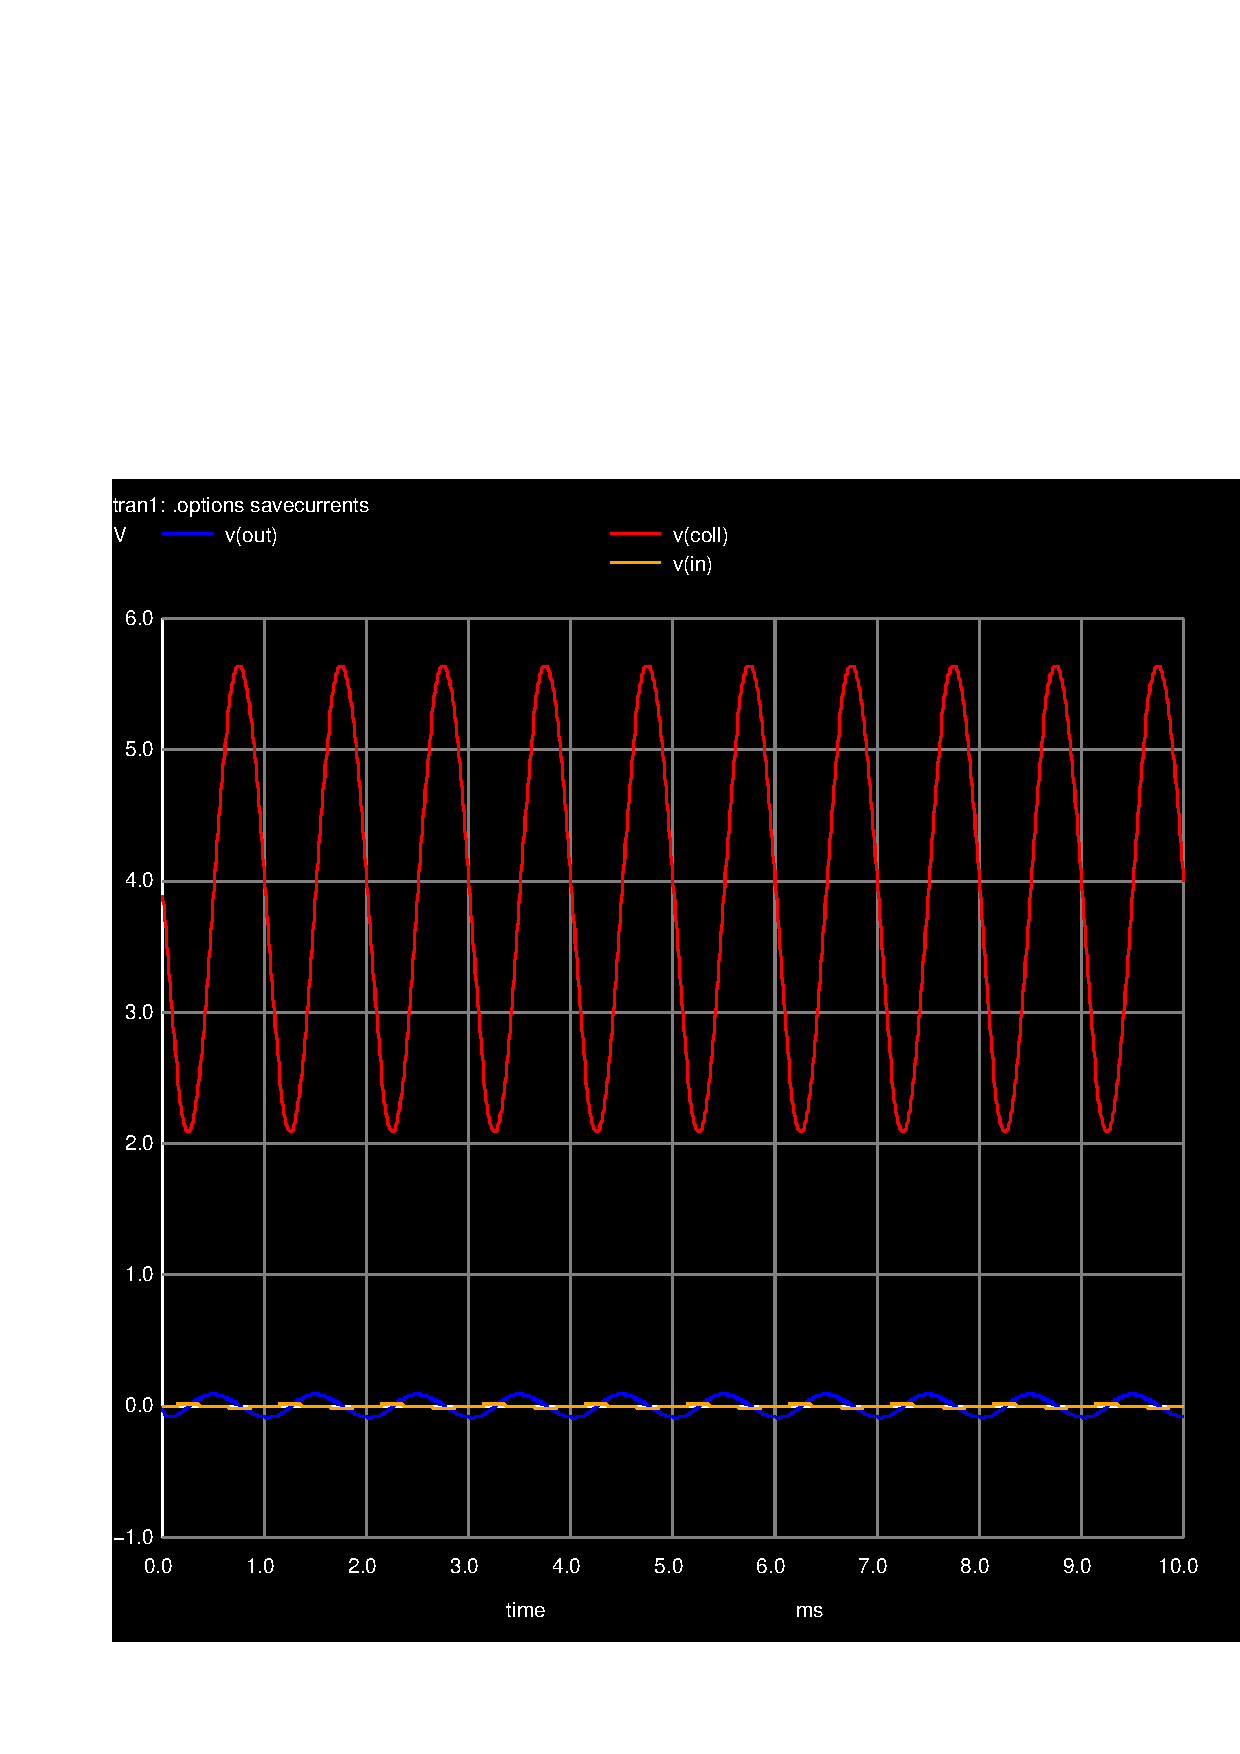
\includegraphics[width=0.5\linewidth]{vo1.pdf}
\caption{Comparison between the input and the output sinusoidal signals.}
\label{fig:comp}
\end{figure}
\par
\begin{table}[h!]
  \centering
  \begin{tabular}{|l|r|}
    \hline    
    {\bf Name} & {\bf Values} \\ \hline
    \input{merit_tab} 
  \end{tabular}
  \caption{Cost and merit of the OP-AMP band-pass filter.}
  \label{tab:merit}
\end{table}

\pagebreak
